\documentclass[11pt]{article}
\usepackage[margin=1in]{geometry}
\usepackage{amsmath,amssymb,amsthm,mathtools,booktabs,array,enumitem}
\usepackage{tikz}
\usetikzlibrary{arrows.meta,positioning,calc}
\usepackage[hidelinks]{hyperref}
\usepackage[nameinlink,noabbrev]{cleveref}

\newtheorem{theorem}{Theorem}
\newtheorem{lemma}[theorem]{Lemma}
\newtheorem{proposition}[theorem]{Proposition}
\newtheorem{corollary}[theorem]{Corollary}
\theoremstyle{remark}
\newtheorem{remark}[theorem]{Remark}
\crefname{theorem}{theorem}{theorems}
\Crefname{theorem}{Theorem}{Theorems}
\crefname{lemma}{lemma}{lemmas}
\Crefname{lemma}{Lemma}{Lemmas}
\crefname{proposition}{proposition}{propositions}
\Crefname{proposition}{Proposition}{Propositions}
\crefname{corollary}{corollary}{corollaries}
\Crefname{corollary}{Corollary}{Corollaries}
\crefname{remark}{remark}{remarks}
\Crefname{remark}{Remark}{Remarks}

\newcommand{\Q}{\mathbb{Q}}
\newcommand{\apl}{\alpha_{\mathrm{pl}}}
\newcommand{\flow}{\operatorname{flow}}
\newcommand{\cost}{\operatorname{cost}}
\newcommand{\Epath}{P^{\mathrm E}}
\newcommand{\Cpath}{P^{\mathrm C}}

\title{A Four-Terminal Planar Lower Bound and a Sharp Equal-Cost Gadget for\\
Cost-Preserving Unsplittable-Flow Rounding}
\author{Matthew Protti}
\date{23 July 2026 --- revision 5}

\begin{document}
\maketitle

\begin{center}
\fbox{\parbox{0.92\textwidth}{\small
This is an unrefereed research disclosure.  Its mathematical claim is
deliberately narrower than ``the exact constant'': it gives a lower bound for
an existential, upper-only, cost-preserving planar rounding constant and a
sharp theorem only inside an explicitly restricted model.  Novelty searches
are ongoing and are not exhaustive.}}
\end{center}

\begin{abstract}
For a planar acyclic single-source unsplittable-flow instance with fractional
arc-load vector $x$, maximum demand $d_{\max}$, and nonnegative arc-cost
vector $c$, let $\apl$ be the least universal factor for which there always
exists an unsplittable routing $y$ satisfying
$c^\top y\le c^\top x$ and $y(a)\le x(a)+\apl d_{\max}$ on every arc.
We give a four-terminal planar family proving
\[
 \apl\ge L:=\frac{299-41\sqrt{41}}{32}
 =1.139747070789\ldots .
\]
The bound is a supremal family bound: for every $\eta>0$ we give a rational
instance requiring an overload larger than $(L-\eta)d_{\max}$.  We also give
an attained integer certificate of $335/294=1.139455782312\ldots$.  Finally,
we prove that $L$ is the exact supremum for the fixed four-terminal topology
when every full expensive choice has equal cost and cost feasibility forces
at least two cheap choices.  The known planar theorem gives the algorithmic,
two-sided upper bound $\apl\le2$.
\end{abstract}

\section{Definitions and scope}

Let $G=(V,A)$ be a finite directed graph, let $s\in V$ be a source, and let
$T\subseteq V\setminus\{s\}$ be terminals with demands
$d=(d_t)_{t\in T}\in\Q_{>0}^T$.  A splittable flow may be specified by
nonnegative path amounts $\lambda_{t,P}$ satisfying
\[
 \sum_{P\text{ an }s\text{--}t\text{ path}}\lambda_{t,P}=d_t
 \qquad(t\in T).
\]
Its aggregate arc loads are
\[
 x(a)=\sum_{t\in T}\sum_{P\ni a}\lambda_{t,P}.
\]
An unsplittable routing $\mathcal P=(P_t)_{t\in T}$ chooses one $s$--$t$
path for every terminal, and has aggregate loads
\[
 \flow_{\mathcal P}(a)=\sum_{t\in T:a\in P_t}d_t.
\]
For $c\in\Q_{\ge0}^A$, define
$\cost_c(z):=\sum_{a\in A}c(a)z(a)$ and
$d_{\max}:=\max_{t\in T}d_t$.

Following the planar convention in Traub--Vargas Koch--Zenklusen, call
$(G,s,T,d,x)$ a planar SSUF instance when $G$ is acyclic and planar.  Define
\begin{align*}
\apl:=\inf\bigl\{\alpha\ge0:\;&\text{for every planar SSUF instance }
 (G,s,T,d,x)\text{ and every }c\in\Q_{\ge0}^A,\\[-1mm]
&\text{there exists an unsplittable }\mathcal P\text{ such that }
\cost_c(\flow_{\mathcal P})\le\cost_c(x)\\[-1mm]
&\text{and }\flow_{\mathcal P}(a)\le x(a)+\alpha d_{\max}
\text{ for every }a\in A\bigr\}.
\end{align*}
This is an \emph{existential} and \emph{upper-only} constant.  It is distinct
from an algorithmic constant and from the cost-free, two-sided discrepancy
question of Morell and Skutella.  The algorithmic theorem of
Traub--Vargas Koch--Zenklusen gives the stronger two-sided estimate
$|\flow_{\mathcal P}(a)-x(a)|\le2d_{\max}$ while preserving cost, and hence
implies $\apl\le2$.

\section{The fixed planar digraph}

Let
\[
 V=\{s=v_0,v_1,v_2,v_3,v_4,v_5,t_1,t_2,t_3,t_4\}.
\]
For $j\in\{1,\dots,5\}$ write $a_j=(v_{j-1},v_j)$.  The arc set is
\begin{align*}
 A={}&\{a_j:1\le j\le5\}\\
 &\cup\{(s,t_1),(v_3,t_1),(s,t_2),(v_5,t_2),
 (v_1,t_3),(v_5,t_3),(v_2,t_4),(v_4,t_4)\}.
\end{align*}
These are all the arcs; in particular, every $t_i$ is a sink.

Each terminal has two designated paths:
\begin{align*}
\Epath_1&=(s,t_1),
&\Cpath_1&=(s,v_1,v_2,v_3,t_1),\\
\Epath_2&=(s,t_2),
&\Cpath_2&=(s,v_1,v_2,v_3,v_4,v_5,t_2),\\
\Epath_3&=(s,v_1,t_3),
&\Cpath_3&=(s,v_1,v_2,v_3,v_4,v_5,t_3),\\
\Epath_4&=(s,v_1,v_2,t_4),
&\Cpath_4&=(s,v_1,v_2,v_3,v_4,t_4).
\end{align*}
The superscripts E and C will stand for expensive and cheap once costs are
introduced.

\begin{figure}[ht]
\centering
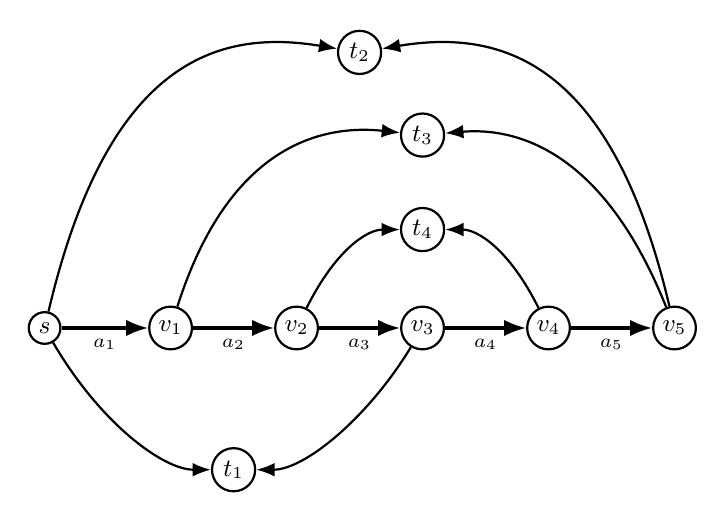
\begin{tikzpicture}[>=Latex,thick,
  vtx/.style={circle,draw,fill=white,inner sep=2pt,font=\small},
  arr/.style={->},
  trunk/.style={->,line width=1.1pt}]
  \node[vtx] (s)  at (0,0) {$s$};
  \node[vtx] (v1) at (1.6,0) {$v_1$};
  \node[vtx] (v2) at (3.2,0) {$v_2$};
  \node[vtx] (v3) at (4.8,0) {$v_3$};
  \node[vtx] (v4) at (6.4,0) {$v_4$};
  \node[vtx] (v5) at (8.0,0) {$v_5$};
  \foreach \u/\v/\lab in {s/v1/a_1,v1/v2/a_2,v2/v3/a_3,v3/v4/a_4,v4/v5/a_5}
    \draw[trunk] (\u)--node[below,font=\scriptsize]{$\lab$}(\v);

  \node[vtx] (t1) at (2.4,-1.8) {$t_1$};
  \node[vtx] (t2) at (4.0,3.5) {$t_2$};
  \node[vtx] (t3) at (4.8,2.45) {$t_3$};
  \node[vtx] (t4) at (4.8,1.25) {$t_4$};

  \draw[arr] (s) .. controls (0.7,-1.2) and (1.5,-1.8) .. (t1);
  \draw[arr] (v3) .. controls (4.1,-1.15) and (3.3,-1.8) .. (t1);

  \draw[arr] (s) .. controls (0.8,3.4) and (2.2,3.8) .. (t2);
  \draw[arr] (v5) .. controls (7.2,3.4) and (5.8,3.8) .. (t2);

  \draw[arr] (v1) .. controls (2.3,2.2) and (3.4,2.6) .. (t3);
  \draw[arr] (v5) .. controls (7.1,2.25) and (6.0,2.55) .. (t3);

  \draw[arr] (v2) .. controls (3.7,1.0) and (4.1,1.25) .. (t4);
  \draw[arr] (v4) .. controls (5.9,1.0) and (5.5,1.25) .. (t4);
\end{tikzpicture}
\caption{The fixed digraph.  The edge list, rather than the drawing, is the
formal specification.}
\label{fig:graph}
\end{figure}

\begin{lemma}\label{lem:graph}
The graph $G$ is a planar DAG, and $\Epath_i,\Cpath_i$ are exactly the two
$s$--$t_i$ paths for each $i\in\{1,2,3,4\}$.
\end{lemma}
\begin{proof}
The order
$s,v_1,v_2,v_3,v_4,v_5,t_1,t_2,t_3,t_4$ is topological.  A plane embedding is
shown in \cref{fig:graph}; equivalently, a clockwise rotation system is
\begin{align*}
&s:(v_1,t_2,t_1),\quad v_1:(s,v_2,t_3),\quad
v_2:(v_1,v_3,t_4),\quad v_3:(v_2,t_1,v_4),\\
&v_4:(v_3,v_5,t_4),\quad v_5:(v_4,t_2,t_3),\quad
 t_1:(v_3,s),\ t_2:(v_5,s),\ t_3:(v_5,v_1),\ t_4:(v_4,v_2).
\end{align*}
Face tracing gives five faces, and $|V|-|A|+5=10-13+5=2$.
Finally, every terminal has precisely the two listed in-neighbors, and the
trunk gives the unique path from $s$ to each such predecessor.  Thus there
are exactly two source-terminal paths.
\end{proof}

The sets used in the discrepancy calculation are not the complete cheap
paths.  They are the supports on the trunk of the path differences:
\[
 I_i:=\{a_j:\mathbf 1_{\Cpath_i}(a_j)-
                    \mathbf 1_{\Epath_i}(a_j)=1\}.
\]
Explicitly,
\[
 I_1=\{a_1,a_2,a_3\},\quad
 I_2=\{a_1,a_2,a_3,a_4,a_5\},\quad
 I_3=\{a_2,a_3,a_4,a_5\},\quad
 I_4=\{a_3,a_4\}.
\]
For example, both paths to $t_3$ use $a_1$, so $a_1\notin I_3$.

\begin{remark}[The graph is outside the series-parallel positive class]
The underlying undirected graph has a $K_4$ minor with connected branch sets
\[
 \{s,t_1,t_2\},\qquad
 \{v_1,v_2,t_3,t_4\},\qquad
 \{v_3,v_4\},\qquad
 \{v_5\}.
\]
Every two branch sets are adjacent.  In particular, the underlying
undirected graph is not two-terminal series-parallel, since such graphs are
$K_4$-minor-free.  Thus the example lies outside the recursively constructed
series-parallel digraph class used by Almoghrabi--Skutella--Warode and does not
conflict with their strict $d_{\max}$ deviation theorem.
\end{remark}

\section{The rational parametric family}

Fix
\[
 q\in(\sqrt3-1,1)\cap\Q,
 \qquad
 \varepsilon\in\Q,
 \qquad
 0<\varepsilon<3-2q-q^2.
\]
Set
\[
 (d_1,d_2,d_3,d_4)=(1,q^2,q,1)
\]
and route the fraction $p_i$ of terminal $i$'s demand on $\Cpath_i$, where
\[
 p_1=1-q^2,\qquad
 p_2=q^2+2q-2+\varepsilon,\qquad
 p_3=p_4=1-q.
\]
The parameter restrictions imply $0<p_i<1$ for every $i$.  Indeed,
$q>\sqrt3-1$ gives $q^2+2q-2>0$, while the upper bound on $\varepsilon$
gives $p_2<1$.  Also
\[
 \sum_{i=1}^4p_i=1+\varepsilon,
 \qquad d_{\max}=1.
\]

Costs are specified on arcs, not assigned abstractly to paths.  Put
\[
 c(s,t_1)=1,\qquad c(s,t_2)=\frac1{q^2},\qquad
 c(v_1,t_3)=\frac1q,\qquad c(v_2,t_4)=1,
\]
and put cost zero on every other arc.  These four charged arcs occur only on
the corresponding expensive paths.  Consequently
\[
 c(\Epath_i)=\frac1{d_i},\qquad c(\Cpath_i)=0,
\]
so routing all of demand $d_i$ expensively costs one.

Let $x$ be the splittable flow that sends $d_ip_i$ on $\Cpath_i$ and
$d_i(1-p_i)$ on $\Epath_i$.

\begin{lemma}[Cost forcing]\label{lem:cost}
The fractional cost is $\cost_c(x)=3-\varepsilon$.  Every unsplittable
routing of cost at most $\cost_c(x)$ chooses at least two cheap paths.
\end{lemma}
\begin{proof}
Terminal $i$ contributes
\[
 d_i(1-p_i)c(\Epath_i)=d_i(1-p_i)\frac1{d_i}=1-p_i
\]
to the fractional cost.  Hence
$\cost_c(x)=\sum_i(1-p_i)=3-\varepsilon$.
An unsplittable routing has cost equal to its integer number of expensive
choices.  Since $3-\varepsilon<3$, a cost-nonincreasing routing uses at most
two expensive paths and therefore at least two cheap paths.
\end{proof}

For a cheap-set $S\subseteq\{1,2,3,4\}$, let $y^S$ denote the unsplittable
routing that uses $\Cpath_i$ exactly for $i\in S$.

\begin{lemma}[Monotonicity on the trunk]\label{lem:monotone}
If $S\subseteq S'$, then
\[
 \flow_{y^{S'}}(a)-x(a)\ge \flow_{y^S}(a)-x(a)
 \qquad\text{for every trunk arc }a.
\]
In particular, every routing with at least three cheap choices
coordinatewise dominates, on the trunk, a routing with exactly two cheap
choices.
\end{lemma}
\begin{proof}
Switching terminal $i$ from $\Epath_i$ to $\Cpath_i$ changes the trunk load by
$d_i\mathbf 1_{I_i}$, which is coordinatewise nonnegative.  Apply such
switches one at a time.
\end{proof}

On an arc of $I_i$, the overload contribution relative to $x$ is
$d_i(1-p_i)$ when $i$ is cheap and $-d_ip_i$ when $i$ is expensive.  These
values are
\[
\begin{array}{c@{\qquad}c@{\qquad}c}
\toprule
 i&\text{cheap contribution}&\text{expensive contribution}\\
\midrule
1&q^2&q^2-1\\
2&q^2(3-q^2-2q-\varepsilon)&-q^2(q^2+2q-2+\varepsilon)\\
3&q^2&q^2-q\\
4&q&q-1\\
\bottomrule
\end{array}
\]
Define
\[
 R(q,\varepsilon):=q^2(4-q^2-2q-\varepsilon).
\]
For the six exactly-two-cheap routings, direct substitution gives:
\[
\begin{array}{c@{\qquad}c@{\qquad}c}
\toprule
S&\text{witness arc}&\flow_{y^S}(a)-x(a)\\
\midrule
\{1,2\}&a_1&R(q,\varepsilon)\\
\{1,3\}&a_2&R(q,\varepsilon)\\
\{1,4\}&a_3&R(q,\varepsilon)\\
\{2,3\}&a_5&R(q,\varepsilon)\\
\{2,4\}&a_4&R(q,\varepsilon)\\
\{3,4\}&a_4&R(q,\varepsilon)+q-q^2\\
\bottomrule
\end{array}
\]
Since $q-q^2>0$, every row is at least $R(q,\varepsilon)$.

\begin{proposition}\label{prop:family}
For every admissible rational pair $(q,\varepsilon)$, every
cost-nonincreasing unsplittable routing overloads some arc by at least
$R(q,\varepsilon)d_{\max}=R(q,\varepsilon)$.
\end{proposition}
\begin{proof}
By \cref{lem:cost}, every cost-nonincreasing routing has at least two cheap
choices.  If it has exactly two, use the table above.  If it has more, use
\cref{lem:monotone} and retain any two of its cheap choices.
\end{proof}

\begin{theorem}\label{thm:main}
\[
 \apl\ge L:=\frac{299-41\sqrt{41}}{32}
 =1.139747070789\ldots .
\]
More precisely, for every $\eta>0$ there is a rational four-terminal planar
SSUF instance for which every cost-nonincreasing unsplittable routing
overloads some arc by more than $(L-\eta)d_{\max}$.
\end{theorem}
\begin{proof}
At $\varepsilon=0$, write
\[
 f(q):=R(q,0)=q^2(4-q^2-2q).
\]
Then
\[
 f'(q)=2q(4-3q-2q^2).
\]
The unique maximizer in $(\sqrt3-1,1)$ is
\[
 q_*=\frac{\sqrt{41}-3}{4},
\]
and direct substitution gives
\[
 f(q_*)=\frac{299-41\sqrt{41}}{32}=L.
\]

Fix $\eta>0$.  By continuity of $f$ and density of the rationals, choose
$q\in(\sqrt3-1,1)\cap\Q$ such that
$f(q)>L-\eta/2$.  Then choose rational $\varepsilon$ satisfying
\[
 0<\varepsilon<\min\left\{3-2q-q^2,\frac{\eta}{2q^2}\right\}.
\]
The instance is admissible, all of its data are rational, and
\[
 R(q,\varepsilon)=f(q)-q^2\varepsilon>L-\eta.
\]
Now apply \cref{prop:family}.  Since this holds for every $\eta>0$, no
universal factor below $L$ can satisfy the definition of $\apl$.
\end{proof}

\begin{corollary}
\[
 \frac{299-41\sqrt{41}}{32}\le\apl\le2.
\]
\end{corollary}
\begin{proof}
The lower bound is \cref{thm:main}.  The upper bound follows from the
cost-preserving two-sided $2d_{\max}$ planar rounding theorem of
Traub--Vargas Koch--Zenklusen.
\end{proof}

\section{Sharpness within an equal-full-cost two-cheap model}

The construction above is tuned, but not arbitrary.  In this section we
show that it is optimal within a precise fixed-topology model.

Keep the digraph and the two paths per terminal from \cref{fig:graph}.
The real relaxation of the model consists of demands
$d\in(0,1]^4$ with $\max_i d_i=1$, cheap fractions $p\in[0,1]^4$, and a
number $K>0$ satisfying
\[
 1<\sum_{i=1}^4 p_i\le2.
\]
Give every cheap path cost zero by charging only the private arc of the
corresponding expensive path, at per-unit cost $K/d_i$.  Thus every full
expensive choice costs $K$.  The fractional cost is
$K(4-\sum_i p_i)\in[2K,3K)$, so a routing is cost-nonincreasing exactly when
it has at least two cheap choices.

For these real data let $x$ send $d_ip_i$ cheaply and $d_i(1-p_i)$
expensively, and let $\beta_G^{\mathrm{eq},2}$ be the supremum of
\[
 \min_{S\subseteq\{1,2,3,4\}:\,|S|\ge2}
 \max_{a\in A}\bigl(\flow_{y^S}(a)-x(a)\bigr).
\]
The superscript records the equal-full-cost and two-cheap regime.  This is a
restricted fixed-topology constant; it does not permit unequal full-route
costs.  Write $\beta_{G,\Q}^{\mathrm{eq},2}$ for the same supremum with
$d,p\in\Q^4$ (and, without loss of generality, rational $K>0$).

\begin{theorem}[Sharpness in the restricted model]\label{thm:sharp-model}
\[
 \beta_G^{\mathrm{eq},2}
 =\beta_{G,\Q}^{\mathrm{eq},2}
 =\frac{299-41\sqrt{41}}{32}=L.
\]
\end{theorem}
\begin{proof}
The family in \cref{prop:family,thm:main} has equal full expensive-route
costs and $\sum_i p_i=1+\varepsilon\in(1,2)$, so it proves
$\beta_G^{\mathrm{eq},2}\ge L$.  We prove the reverse inequality.

Fix arbitrary data in the restricted model.  Decrease the cheap fractions
coordinatewise, if necessary, to numbers $\widehat p_i\le p_i$ satisfying
$\sum_i\widehat p_i=1$.  For every exactly-two-cheap routing and every trunk
arc, this change can only increase the deviation from the fractional flow:
for a cheap terminal the contribution changes from $d_i(1-p_i)$ to
$d_i(1-\widehat p_i)$, and for an expensive terminal it changes from
$-d_ip_i$ to $-d_i\widehat p_i$.  Thus an upper bound for the boundary data
$\widehat p$ is also an upper bound for the original data.  Every
exactly-two-cheap routing is cost-feasible in the original instance.

Write
\[
 \ell_i:=d_i\widehat p_i,
 \qquad
 e_i:=d_i(1-\widehat p_i).
\]
Positive deviations on private terminal arcs are at most $d_i\le1$, so only
trunk deviations can matter for a bound larger than one.  Let $M_{ij}$ be
the maximum trunk deviation when precisely terminals $i$ and $j$ are cheap.
Directly from the four difference supports $I_i$,
\[
\begin{array}{c@{\qquad}c}
\toprule
\{i,j\}&M_{ij}\\
\midrule
\{1,2\}&e_1+e_2\\
\{1,3\}&e_1+e_3-\ell_2\\
\{1,4\}&\max\{e_1-\ell_2,\ e_1+e_4-\ell_2-\ell_3\}\\
\{2,3\}&e_2+e_3\\
\{2,4\}&\max\{e_2-\ell_1,\ e_2+e_4-\ell_3\}\\
\{3,4\}&e_3+e_4-\ell_2\\
\bottomrule
\end{array}
\]
If $e_4<\ell_3$, then $M_{14}=e_1-\ell_2\le1$, and we are done.  Hence
assume $e_4\ge\ell_3$.  In that case
\[
 M_{14}=e_1+e_4-\ell_2-\ell_3,
 \qquad
 M_{24}=e_2+e_4-\ell_3.
\]
Because $d_1,d_4\le1$,
\[
 \widehat p_1=1-\frac{e_1}{d_1}\le1-e_1,
 \qquad
 \widehat p_4\le1-e_4.
\]
Using $\sum_i\widehat p_i=1$ gives
\begin{equation}\label{eq:e14-bound}
 e_1+e_4\le1+\widehat p_2+\widehat p_3.
\end{equation}

Put
\[
 s:=d_2,\quad t:=d_3,\quad p:=\widehat p_2,\quad q:=\widehat p_3.
\]
Thus $0<s,t\le1$, $p,q\ge0$, and $p+q\le1$, while
\[
 e_2=s(1-p),\quad \ell_2=sp,
 \qquad
 e_3=t(1-q),\quad \ell_3=tq.
\]
Define
\[
 L_0:=\min\{e_2,e_3-\ell_2\},
 \qquad
 R_0:=\min\{e_2-\ell_3,e_3-\ell_2\}.
\]
The first two rows involving terminal 1 have minimum $e_1+L_0$, while the
last two rows involving terminal 4 have minimum $e_4+R_0$.  Therefore,
using \eqref{eq:e14-bound},
\begin{equation}\label{eq:T-bound}
 \min_{|S|=2}M_S\le\min\{T_1,T_2,T_3\},
\end{equation}
where
\[
 T_1:=e_2+e_3,
 \qquad
 T_2:=1+p+q-\ell_2-\ell_3,
 \qquad
 T_3:=\frac{1+p+q+L_0+R_0}{2}.
\]
Indeed, $T_1=M_{23}$, $M_{14}\le T_2$, and the minimum of
$e_1+L_0$ and $e_4+R_0$ is at most their average.

First suppose $t\ge s$.  The difference between the two candidates in
$R_0$ is
\[
 (e_3-\ell_2)-(e_2-\ell_3)=t-s,
\]
so $R_0=e_2-\ell_3$.  Also,
$L_0=e_2$ when $e_3\ge s$, and $L_0=e_3-\ell_2$ when $e_3\le s$.
Consequently $T_3$ is at most
\[
 \widetilde T_3
 :=\frac{1+2s+(1-2s)p+(1-t)q}{2}.
\]
If $e_3\ge s$ then equality holds; if $e_3\le s$, the difference
$\widetilde T_3-T_3$ is $(s-e_3)/2\ge0$.

If $s+s/t\le1$, then $s\le1/2$ and
\[
 (1-2s)T_1+2s\widetilde T_3
 =t+2s(1-t)+q\bigl(s(1+t)-t\bigr)\le1.
\]
Indeed, $s\le t/(1+t)$ makes the coefficient of $q$ nonpositive, while
\[
 t+2s(1-t)\le t+\frac{2t(1-t)}{1+t}
 =\frac{t(3-t)}{1+t}\le1.
\]
The coefficients on the left are nonnegative and sum to one, so
\eqref{eq:T-bound} is at most one.

Now assume $s+s/t\ge1$.  Set
\[
 \lambda_1:=\frac{s}{t}-s,
 \qquad
 \lambda_2:=s+\frac{s}{t}-1,
 \qquad
 \lambda_3:=2\left(1-\frac{s}{t}\right).
\]
These numbers are nonnegative and sum to one.  A direct cancellation gives
\[
 \lambda_1T_1+\lambda_2T_2+\lambda_3\widetilde T_3
 =g(s,t):=s\left(4-s-t-\frac{s}{t}\right).
\]
Hence the right-hand side of \eqref{eq:T-bound} is at most $g(s,t)$.

It remains to consider $t\le s$.  Now both minima in $L_0$ and $R_0$ select
$e_3-\ell_2$, and hence
\[
 T_3=\frac{1+2t+(1-2s)p+(1-2t)q}{2}.
\]
If $t\le1/2$, then
\[
 (1-2t)T_1+2tT_3
 =s+2t-2st+p(t-s)\le1.
\]
Here $p(t-s)\le0$ and
$s+2t(1-s)\le s+(1-s)=1$.
If $t\ge1/2$, then
\[
 (2t-1)T_2+2(1-t)T_3
 =t(3-2t)+p(t-s)\le t(3-2t)\le\frac98.
\]
Again $p(t-s)\le0$, and the displayed coefficients are nonnegative and sum
to one.

Thus a value above $9/8$ can occur only in the region
\[
 0<s\le t\le1,
 \qquad
 s+\frac{s}{t}\ge1,
\]
and there it is at most $g(s,t)$.  Equivalently, optimize on the compact set
\[
 \overline{\mathcal D}:=
 \{(s,t):0\le s\le t\le1,\ s(t+1)\ge t\}.
\]
The only point with $t=0$ is $(0,0)$.  Defining $g(0,0)=0$ makes $g$
continuous there, because $0\le s^2/t\le s$ whenever $0<s\le t$.
The unique interior stationary point of $g$ satisfies
\[
 s=t^2,
 \qquad
 2t^2+3t-4=0,
\]
so
\[
 t=\frac{\sqrt{41}-3}{4},
 \qquad
 s=t^2,
 \qquad
 g(s,t)=L.
\]
On the three nontrivial boundary pieces,
\[
\begin{array}{c@{\qquad}c}
 s=t&g=t(3-2t)\le9/8,\\
 t=1&g=s(3-2s)\le9/8,\\
 s+s/t=1&g=\dfrac{t(3-t)}{t+1}\le1.
\end{array}
\]
(The remaining boundary point is $(0,0)$ and has value zero.)  Since
$L>9/8$ (equivalently $263>41\sqrt{41}$), the global maximum is $L$.
Therefore every instance in the restricted model has a
cost-feasible routing with overload at most $L$, proving the upper bound.
The rational family from \cref{thm:main} approaches $L$, so imposing rational
data does not change the supremum.
\end{proof}

\begin{remark}
Theorem~\ref{thm:sharp-model} does not cover unequal full expensive-route
costs, a different cost threshold requiring three or four cheap choices, or
other four-terminal topologies.  Those remain separate optimization
questions.
\end{remark}

\section{A finite integer certificate: \texorpdfstring{$335/294$}{335/294}}

Choose
\[
 q=\frac67,
 \qquad
 \varepsilon=\frac1{10584},
\]
so that
\[
 (p_1,p_2,p_3,p_4)=
 \left(\frac{13}{49},\frac{97}{216},\frac17,\frac17\right),
 \qquad
 \sum_i p_i=1+\frac1{10584}.
\]
Scale all demands and path amounts by $294$.  The resulting integer data are
\[
\begin{array}{c@{\qquad}r@{\qquad}r@{\qquad}r}
\toprule
 i&d_i&\text{cheap amount}&\text{expensive amount}\\
\midrule
1&294&78&216\\
2&216&97&119\\
3&252&36&216\\
4&294&42&252\\
\bottomrule
\end{array}
\]
and $d_{\max}=294$.

Let $M=10584$.  Put per-unit costs
\[
 36=\frac{M}{294},
 \qquad
 49=\frac{M}{216},
 \qquad
 42=\frac{M}{252},
 \qquad
 36=\frac{M}{294}
\]
on $(s,t_1),(s,t_2),(v_1,t_3),(v_2,t_4)$, respectively, and zero on every
other arc.  Thus each full expensive choice costs $M$.  The fractional cost
is
\begin{align*}
\cost_c(x)
 &=216(36)+119(49)+216(42)+252(36)\\
 &=31751
 =3M-1
 <3M=31752.
\end{align*}
Therefore every cost-nonincreasing unsplittable routing has at least two
cheap choices.

For completeness, the fractional load on every arc is
\[
\begin{array}{c@{\quad}r@{\qquad}c@{\quad}r}
\toprule
\text{arc}&x(a)&\text{arc}&x(a)\\
\midrule
 a_1&721&(s,t_1)&216\\
 a_2&505&(v_3,t_1)&78\\
 a_3&253&(s,t_2)&119\\
 a_4&175&(v_5,t_2)&97\\
 a_5&133&(v_1,t_3)&216\\
 &&(v_5,t_3)&36\\
 &&(v_2,t_4)&252\\
 &&(v_4,t_4)&42\\
\bottomrule
\end{array}
\]
Flow conservation at the nonterminals follows from
\[
\begin{aligned}
721+216+119&=1056=294+216+252+294,\\
721&=505+216,\qquad 505=253+252,\\
253&=175+78,\qquad 175=133+42,\qquad 133=97+36.
\end{aligned}
\]

The six exactly-two-cheap cases are
\[
\begin{array}{c@{\qquad}c@{\qquad}r}
\toprule
S&\text{witness arc}&\flow_{y^S}(a)-x(a)\\
\midrule
\{1,2\}&a_1&335\\
\{1,3\}&a_2&335\\
\{1,4\}&a_3&335\\
\{2,3\}&a_5&335\\
\{2,4\}&a_4&335\\
\{3,4\}&a_4&371\\
\bottomrule
\end{array}
\]
Together with \cref{lem:monotone}, this covers all eleven cost-feasible
routings.  Hence this single integer instance proves
\[
 \apl\ge\frac{335}{294}=1.139455782312\ldots.
\]
The lower bound is attained as the exact minimum maximum overload among the
cost-feasible routings.  For example, the routing with cheap set $\{1,2\}$
has full deviation vector
\[
\begin{aligned}
 (a_1,\ldots,a_5)&=(335,299,257,41,83),\\
 ((s,t_1),(v_3,t_1))&=(-216,216),\\
 ((s,t_2),(v_5,t_2))&=(-119,119),\\
 ((v_1,t_3),(v_5,t_3))&=(36,-36),\\
 ((v_2,t_4),(v_4,t_4))&=(42,-42).
\end{aligned}
\]
Its maximum deviation is exactly $335$.  Positive deviations on private
terminal arcs are at most $252<d_{\max}$.

\begin{remark}[Binary arc costs]
If costs in $\{0,1\}$ are preferred, replace the four charged private arcs
of cost $36,49,42,36$ by directed paths of the corresponding lengths, with
unit cost on every replacement arc.  This preserves acyclicity, planarity,
the two-route structure, all path costs, and the certificate.
\end{remark}

\section{What is and is not proved}

The radical $L$ is the exact maximum of the one-variable limiting function
$q^2(4-q^2-2q)$ and, by \cref{thm:sharp-model}, the exact supremum for the
specified equal-full-cost two-cheap model on the fixed topology.  We do
\emph{not} claim that it is the exact value of $\apl$, the exact unrestricted
four-terminal constant, the optimum on the fixed topology with unequal
full-route costs, or the best four-terminal planar gadget.  The result is
also not an algorithmic lower bound in any special sense: it is an
existential obstruction, and therefore applies a fortiori to any
algorithmic version of the constant.

The supplementary verifier is not needed for the proof.  It reconstructs the
two paths per terminal from the edge list, checks connectedness and that a
supplied rotation system defines a genus-zero embedding, verifies acyclicity,
flow conservation, and legal arc costs, and enumerates all $16$ unsplittable
routings on all $13$ arcs using exact integer arithmetic.  Separate symbolic
scripts derive the path-difference supports from the graph, verify the family
identities and radical optimization, and audit the convex-combination proof
of \cref{thm:sharp-model}.  Mutation tests confirm that representative changes
to the graph, amounts, costs, rotation system, minor certificate, and expected
overload are rejected.

\section{Research provenance and contemporaneous context}

The investigation was directed by Matthew Protti.  OpenAI GPT-5.6 Pro was
used substantively for construction search, symbolic derivation, proof
development, verifier development, and drafting.  Separate model sessions
and a Codex execution session reimplemented and stress-tested key claims from
the stated graph and numerical data.  These are computational cross-checks,
not independent human verification or peer review.  The author reviewed the
claims, selected the scope of this disclosure, and accepts responsibility for
the released work.

The investigation began after Dmitry Rybin's
\href{https://x.com/dmitryrybin1/status/2079904005652893709}{public post of
22 July 2026} announcing a counterexample to Goemans' cost conjecture.
Because related work is developing rapidly, the novelty statements
accompanying this note are expressly limited to targeted searches.  Private
development prompts and conversation transcripts are not released; the
mathematical proof, explicit instance, and executable checks are intended to
make the claims auditable without them.

\begin{thebibliography}{9}

\bibitem{DGG99}
Y.~Dinitz, N.~Garg, and M.~X.~Goemans,
\emph{On the single-source unsplittable flow problem},
Combinatorica 19 (1999), 17--41.
\href{https://doi.org/10.1007/s004930050043}{doi:10.1007/s004930050043}.

\bibitem{MS22}
S.~Morell and M.~Skutella,
\emph{Single source unsplittable flows with arc-wise lower and upper bounds},
Mathematical Programming 192 (2022), 477--496.
\href{https://doi.org/10.1007/s10107-021-01704-4}{doi:10.1007/s10107-021-01704-4}.

\bibitem{TVZ26}
V.~Traub, L.~Vargas Koch, and R.~Zenklusen,
\emph{Single-source unsplittable flows in planar and bounded-genus graphs},
Mathematical Programming (2026).
\href{https://doi.org/10.1007/s10107-026-02365-x}{doi:10.1007/s10107-026-02365-x}.

\bibitem{AMSW26}
M.~Majthoub Almoghrabi, M.~Skutella, and P.~Warode,
\emph{Integer and unsplittable multiflows in series-parallel digraphs},
Mathematical Programming (2026).
\href{https://doi.org/10.1007/s10107-026-02392-8}{doi:10.1007/s10107-026-02392-8}.

\bibitem{STVZ26}
C.~Swamy, V.~Traub, L.~Vargas Koch, and R.~Zenklusen,
\emph{Unsplittable cost flows from unweighted error-bounded variants},
Proceedings of SOSA 2026, 512--523.
\href{https://doi.org/10.1137/1.9781611978964.42}{doi:10.1137/1.9781611978964.42}.

\end{thebibliography}

\appendix
\section{The six symbolic substitutions}

For auditability, here are the witness calculations without omitted steps.
Let
\[
 b_2:=q^2(q^2+2q-2+\varepsilon).
\]
Then
\begin{align*}
\{1,2\},a_1:\quad
 &q^2+q^2(3-q^2-2q-\varepsilon)=R,\\
\{1,3\},a_2:\quad
 &q^2-b_2+q^2=R,\\
\{1,4\},a_3:\quad
 &q^2-b_2+(q^2-q)+q=R,\\
\{2,3\},a_5:\quad
 &q^2(3-q^2-2q-\varepsilon)+q^2=R,\\
\{2,4\},a_4:\quad
 &q^2(3-q^2-2q-\varepsilon)+(q^2-q)+q=R,\\
\{3,4\},a_4:\quad
 &-b_2+q^2+q=R+q-q^2.
\end{align*}

\end{document}
